\section{Interest Rate Products}
\subsection{Zero Coupon Bonds}
\begin{definition}
    A \textbf{stochastic discount factor} $D(t, T)$ is the price at time t of receiving 1 at time T.

    Consider a deterministic bond $B_t$ with 
    \begin{align*}
        dB_t = r_t B_t dt
    \end{align*}
    then clearly
    \begin{align*}
        B_t = B_0 \cdot e^{\int_{0}^{t} r_s ds} 
    \end{align*}
    letting $B_T = 1$, we have $ B_0 = e^{-\int_{0}^{T} r_s ds} = D(0, T)$, so the stochastic discount factor is the price of a riskless bond that pays 1 at T.
\end{definition}
\begin{definition}
    A \textbf{Zero Coupon Bond} is a bond that pays its Face Value at T. 
    WLOG assume the face value is 1, then its price at t is given by
    \begin{equation}
        P(t, T) = E_Q\left[ e^{-\int_{t}^{T} r_t dt }\right] = E_Q\left[ D(t, T) \right]
        \label{eq:zcb}
    \end{equation}
    where $r_t$ is the short rate at time t, and the expectation is taken with respect to the risk free measure Q.

    Note in the case when $r_t$ is constant, we have
    \begin{align*}
        P(t, T) = E_Q\left[ e^{-r(T - t)} \right] \\
        = e^{-r(T - t)} = D(t, T)
    \end{align*}
\end{definition}

\subsection{Linear, Compound, Short rates and Annual Spot Rates}
\begin{definition}
    The \textbf{Spot Linear / Simply Compounded / LIBOR Rate} $L$ is the rate that pays linear interest. \\
    Basically when you pay X, you are supposed to receive $X(1 + L \cdot n)$ after n years \\
    To receive 1 at T, while paying $P(t, T)$ at time $t$, so the spot rate $L(t, T)$ is given by
    \begin{align*}
        p(t, T) (1 + L \cdot (T - t)) = 1 \\
        L(t, T) = \frac{\frac{1}{P(t, T)} - 1}{T - t} \\
        = \frac{1 - P(t, T)}{P(t, T) \cdot (T - t)}
    \end{align*}

\end{definition}

\begin{definition}
    The \textbf{Spot Compound / Continuous Rate} $R(t, T)$ is the rate that pays continuous interest\\
    Pay X at t and receive $X \cdot e^{R \cdot (T - t)}$ at T \\
    To receive 1 at T, while paying $P(t, T)$ at time $t$: 
    \begin{align*}
        P(t, T) \cdot e^{R \cdot (T - t)} = 1 
    \end{align*}
    so the spot rate $R(t, T)$ is given by
    $$
        R(t, T) = \frac{\log(1/P)}{T - t} = 
        \frac{-\log P(t, T)}{T - t}
    $$
    Note here we have the short rate $r_t = \lim_{t \to T^-}R(t, T) \approx R(t, t)$
\end{definition}

\begin{definition}
With $R(t, T)$, we arrive with the \textbf{short rate} $r_t$:
\begin{align*}
    r_t =& \lim_{T \to t} R(t, T) \\
    =& \lim_{T \to t} \frac{-\log P(t, T)}{T - t} 
\end{align*}
\end{definition}

\begin{definition}
    The \textbf{Annual Spot Rate} $Y$ is the rate that pays interest annually. \\
    Pay X at t and receive $X \cdot (1 + Y)^{T - t}$ at T \\
    We again solve
    \begin{align*}
        P \cdot (1 + Y)^{T - t} = 1
    \end{align*}
    So the spot rate $Y(t, T)$ is given by
    $$
        Y(t, T) = \frac{1}{P^\frac{1}{T - t}} - 1
    $$
    In this case the zero coupon bond price is given by
    $$
        P(t, T) = \frac{1}{(1 + Y)^{T - t}}
    $$
\end{definition}

\begin{definition}
    The \textbf{Zero-Coupon Curve} is the curve given by
$$
    T \mapsto 
\begin{cases} 
    L(t, T), &  T \leq t+1, \\
    Y(t, T), & T > t + 1
\end{cases}
$$
Basically, we use the LIBOR rate for expiry within one year, 
and the annual spot rate for long term rates.

An example of a yield curve in Feb 2025 is given by Figure \ref{fig:yield_curve},
where we note that the yield initially goes down, but goes up when 
maturity $>5Y$.\\
Note the general bond formula for a maturity of N years is given by
\begin{align*}
    P(0, N) = \sum_{n=1}^N \frac{C}{(1 + Y)^n} + \frac{F}{(1 + Y)^N}
\end{align*}
Where C is the coupon payment, and F is the face value.\\
For fixed C and F, when price goes down, yield goes up.\\
The fact that less people demand long term bonds,
causes the yield to go up, as investors expect rates to go up in the long run, 
hence demand higher yield for long term bonds.

\begin{figure}
    \centering
    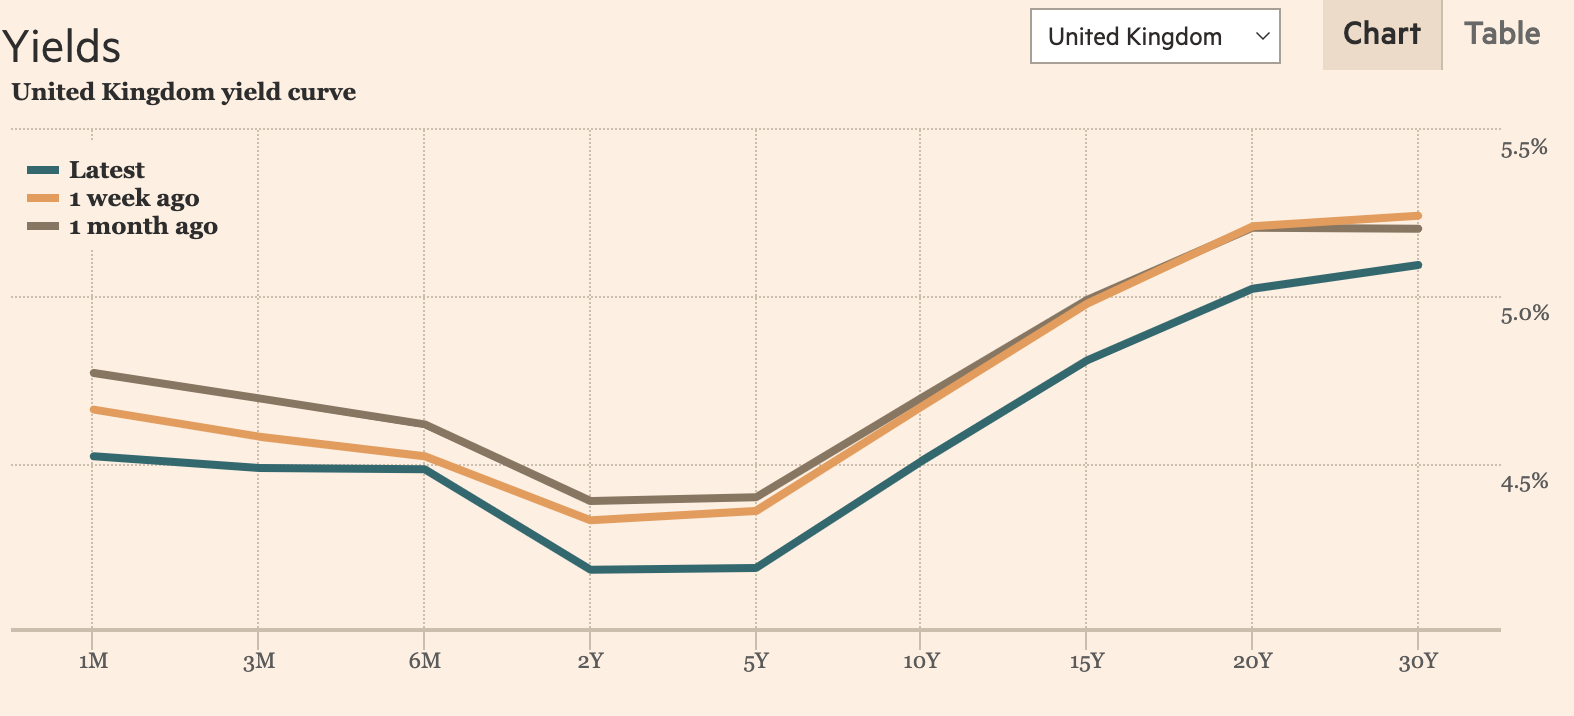
\includegraphics[width=0.8\textwidth]{plots/yield_curve.png}
    \caption{Yield Curve}
    \label{fig:yield_curve}
\end{figure}
\end{definition}

\subsection{Forward Rate}

    A \textbf{Forward Rate Agreement} (FRA) is a contract between two parties, where one party pays a fixed interest rate and the other party pays a floating interest rate. The contract is settled at the end of the contract period.
    
    As we consider at \(t\), the \(\mathrm{FRA}(T_1, T_2)\) is a contract that starts at \(T_1\) and ends at \(T_2\). The fixed rate is agreed at \(T_1\), and settled at \(T_2\). \\
    For the period \(\bigl(T_1, T_2\bigr)\), the holder of the \textbf{Payer FRA} pays fixed \(K \cdot \bigl(T_2 - T_1\bigr)\) and receives floating \(L(T_1, T_2) \cdot \bigl(T_2 - T_1\bigr)\). \\
    The holder of the \textbf{Receiver FRA} has the opposite payoff, with payoff at \(T_2\) given by
    \[
       \bigl(K - L(T_1, T_2)\bigr)\,\bigl(T_2 - T_1\bigr)\,N,
    \]
    where N is the notional amount, and we denote \(\tau = T_2 - T_1\).\\
    Holding 1 at \(T_2\) is equivalent to holding \(P(T_1, T_2)\) at \(T_1\), 
    and holding \(P(t, T_1) P(T_1, T_2)\) at \(t\).\\
    So we can use \(P(t, T_1)\,P(T_1, T_2)\) as the discount factor from \(T_2\) to \(t\).\\
    Note that \(P(T_1, T_2)\) is random at \(t\), and is denoted as 
    the \textbf{Forward Price} \(P(t, T_1, T_2)\) \\
    Recall that we have
    \begin{align*}
        P(T_1, T_2) \bigg( 1 + L(T_1, T_2) \tau  \bigg) = 1 \\
        L(T_1, T_2) = \frac{1}{\tau} \left( \frac{1}{P(T_1, T_2)} - 1 \right) 
    \end{align*}
    Where $P(T_1, T_2)$ is random at t.\\
    Note that we have $D(T_1, T_2) = D(t, T_2) / D(t, T_1)$, but the same doesn't
    hold for the zero coupon bond price $P$. \\
    Nevertheless to price the FRA, we estimate $P(T_1, T_2)$ with $P(t, T_1) P(T_1, T_2)$,
    and have
    \begin{align*}
        \hat{L}(T_1, T_2)
        = \frac{1}{\tau} \left( \frac{P(t, T_1)}{P(t, T_2)} - 1 \right) 
    \end{align*}
    \begin{definition}
    To make the FRA fair, we need 
    \begin{align}
        K \;=\; \hat{L}(T_1, T_2) \;=\; \frac{1}{\tau} \left( \frac{P(t, T_1)}{P(t, T_2)} - 1 \right).
        \label{eq:forward_rate}
    \end{align}
    Which is computable (non-random) at \(t\).\\
    This is the \textbf{Forward Linear Rate} $ F(t, T_1, T_2) $.\\

    \begin{remark}
        \begin{align*}
            P(t, T_1) P(T_1, T_2) = E[D(t, T_1)] E[ D(T_1, T_2)] \neq
            E[D(t, T_1) D(T_1, T_2)] = E[D(t, T_2)] = P(t, T_2)
        \end{align*}
        As we have no evidence that $D(t, T_1)$ and $D(T_1, T_2)$ are uncorrelated.
    \end{remark}
    \end{definition}
    \begin{definition}
    Similarly, we can define the \textbf{Forward Compound Rate} $ R(t, T_1, T_2) $ :\\
    By letting $ K = R(T_1, T_2) $ instead of $ K = L(T_1, T_2) $\\
    Recall
    \begin{align*}
        R(T_1, T_2) = \frac{\,-\log P(T_1, T_2)\,}{\,T_2 - T_1\,}
    \end{align*}
    Writing $ -\log P(T_1, T_2) = -\log P(t, T_1) + \log P(t, T_2) $, we have
    \begin{align}
        R(t, T_1, T_2) \;=\; \frac{\,-\log P(t, T_1) + \log P(t, T_2)\,}{\,T_2 - T_1\,}.
    \label{eq:forward_compound_rate}
    \end{align}
    \end{definition}
    But we continue with the linear / LIBOR rate for now.

    \subsection{FRA}
    Note we derived the forward linear and compound rate above informally,
    by plugging in $P(t, T_1) P(T_1, T_2)$ for $P(t, T_2)$ in the definition of $L(T_1, T_2)$.\\
    This is not rigorous, so we formally derive the price of FRA below,
    and derive the forward rate by setting FRA to 0.
    \begin{definition}
        Assume N = 1. The payoff of the \textbf{Receiver FRA}($t, T_1, T_2$) at \(T_2\)
        is $\tau \, \bigl(K - L(T_1, T_2)\bigr) $\\
        To price it at $t$, we discount the payoff with the factor \(D(t, T_2)\), 
        and take the expectation under \(Q\)
    \begin{align*}
        \mathrm{Receiver\;FRA}(t) 
          &= \tau\; E_Q\bigl[\,D(t, T_2)\,\bigl(K - L(T_1, T_2)\bigr)\bigr]\\
          &= \tau\,K\,E_Q\bigl[\,D(t, T_2)\bigr] - \tau\,E_Q\bigl[\,D(t, T_2)\,L(T_1, T_2)\bigr]\\
          &= \tau\,K\,P\bigl(t, T_2\bigr) - \tau\,E_Q\bigl[\,D(t, T_2)\,L(T_1, T_2)\bigr]
    \end{align*}
    We note that the second term:
    \begin{align*}
        \tau\, E_Q\bigl[\,D(t, T_2)\,L(T_1, T_2)\bigr]
        &= \tau\, E_Q\bigl[\,D(t, T_1) D(T_1, T_2)\,L(T_1, T_2)\bigr]\\
        &= \tau\, E_Q\bigl[ E_T[ D(t, T_1) D(T_1, T_2)\,L(T_1, T_2) ]\bigr]
    \end{align*}
    Where we denote $E_T$ as the expectation taken at $T_1$, 
    (i.e. with the filtration $\mathcal{F}_{T_1}$).\\
    We note that at $T_1$, $D(t, T_1)$ and $L(T_1, T_2)$ are non-random.
    Therefore
    \begin{align*}
        \tau\, E_Q\bigl[\,D(t, T_2)\,L(T_1, T_2)\bigr]
        &= \tau\, E_Q\bigl[ D(t, T_1) L(T_1, T_2) E_T[ D(T_1, T_2) ]\bigr]\\
        &= \tau\, E_Q\bigl[ D(t, T_1) L(T_1, T_2) P(T_1, T_2)\bigr]\\
        &= \tau\, E_Q\bigl[ D(t, T_1) \frac{1}{\tau} 
        \left( \frac{1}{P(T_1, T_2)} - 1 \right) P(T_1, T_2)\bigr]\\
        &= E_Q \bigl[ D(t, T_1) \left( 1 - P(T_1, T_2) \right) \bigr]\\
        &= P(t, T_1) - E_Q \bigl[ D(t, T_1) P(T_1, T_2) \bigr]
    \end{align*}
    Again, note that the second term
    \begin{align*}
        E_Q \bigl[ D(t, T_1) P(T_1, T_2) \bigr]
        &= E_Q \bigl[ D(t, T_1) E_{T_1} [  D(T_1, T_2) ] \bigr]\\
        &= E_Q \bigl[ E_{T_1} [ D(t, T_1) D(T_1, T_2) ] \bigr]\\
        &= E_Q \bigl[ D(t, T_2) \bigr] \\
        &= P(t, T_2)
    \end{align*}
    So we end up with 
    \begin{align}
        \mathrm{Receiver\;FRA}(t) 
        &= \tau\,K\,P\bigl(t, T_2\bigr) - P(t, T_1) + P(t, T_2) \label{eq:fra}
    \end{align}
\end{definition}

We solve FRA(K) = 0, and note that the solution is exactly 
$K = F(t, T_1, T_2) 
= \frac{1}{\tau} \left( \frac{P(t, T_1)}{P(t, T_2)} - 1 \right)$:
\[
   FRA(K) =  \,\Bigl(\,\tau\,K\,P(t, T_2) - P(t, T_1) + P(t, T_2)\Bigr) = 0
\]
\[
   K = \frac{1}{\tau} \left( \frac{P(t, T_1) - P(t, T_2)}{P(t, T_2)} \right)
\]

\begin{definition}
    The \textbf{Instantaneous Forward Rate} $f(t, T)$ is the estimated rate to be paid from T to T + dt, 
    computed by taking the following limit \\
    \begin{align*}
        f(t, T) =& \lim_{\tau \to 0} F(t, T, T + \tau) = \lim_{\tau \to 0} \frac{P(t, T) - P(t, T + \tau)}{P(t, T + \tau) \cdot \tau} \\
        =& \lim_{\tau \to 0} -\frac{1}{P(t, T + \tau)} \cdot \frac{P(t, T + \tau) - P(t, T)}{\tau} 
    \end{align*}
    We note that both terms in the limit has well defined limits, 
    so the limit of the product is the product of the limits. So
    \begin{align*}
        f(t, T) 
        =& -\frac{1}{P(t, T)} \cdot \frac{\partial}{\partial T} P(t, T) \\
        =& -\frac{\partial}{\partial T} \log P(t, T)
    \end{align*}
    This can be viewed as an estimate for the future short rate $r(T)$, which is random at t.
\end{definition}
Note under mild regularity conditions, the instantaneous forward rate should converge to the short rate:
\begin{align*}
    r_t =& \lim_{\tau \to 0} f(t, t + \tau) \\
    =& \lim_{\tau \to 0} -\frac{\partial}{\partial T} \log P(t, T)
\end{align*}
While we previously have
\begin{align*}
    r_t =& \lim_{\tau \to 0} R(t, t + \tau) \\
    =& \lim_{\tau \to 0} -\frac{1}{T} \log P(t, T) 
\end{align*}

Consider a trivial example of a quadratic zero coupon bond.
\begin{align*}
    P(0, T) =& e^{-A T^2 -B T - C} 
\end{align*}
First we note that we need $P(0, 0) = 1$, so $C = 0$.\\
Additionally we need $P(0, T) \in [0, 1)$, so $A \geq 0 \, , B \geq 0$.\\
Then we have
\begin{align*}
    R(0, T) =& -\frac{1}{T} (-A T^2 -B T) = A T + B \\
    r_0 =& R(0, 0) = B
\end{align*}
And
\begin{align*}
    f(0, T) =& -\frac{\partial}{\partial T} \log P(0, T) = 2 A T + B \\
    r_0 =& f(0, 0) = B
\end{align*}
So in this case, the instantaneous forward rate and continuous Compounded rate
agrees in the limit to the short rate

\subsection{Remarks: Forward Rate is an biased estimator}

Note in (2.1) and (2.2), we showed
\[
    \tau \;E_Q\Bigl[D\bigl(t, T_2\bigr)\,\bigl(K - L(T_1, T_2)\bigr)\Bigr]
    \;=\; \tau\,K \,P\bigl(t, T_2\bigr) \;-\; P\bigl(t, T_1\bigr) \;+\; P\bigl(t, T_2\bigr).
\]
Where
\[
    E_Q\Bigl[D\bigl(t, T_2\bigr)\,\bigl(K - L(T_1, T_2)\bigr)\Bigr]
    = K \,P\bigl(t, T_2\bigr) - E_Q\Bigl[D\bigl(t, T_2\bigr)\,L(T_1, T_2)\Bigr].
\]
Hence
\begin{align*}
    P\bigl(t, T_1\bigr) - P\bigl(t, T_2\bigr) 
    =& \tau \Bigl(\,K\,P\bigl(t, T_2\bigr) \;-\; E_Q\bigl[D\bigl(t, T_2\bigr)\,(K - L)\bigr]\Bigr)\\
    =& \tau \Bigl(K \,P\bigl(t, T_2\bigr) - K\,P\bigl(t, T_2\bigr) 
    + E_Q\bigl[D\bigl(t, T_2\bigr)\,L(T_1, T_2)\bigr]\Bigr) \\
    =& \tau\;E_Q\Bigl[D\bigl(t, T_2\bigr)\,L(T_1, T_2)\Bigr]
\end{align*}
So we have
\[
    \frac{P\bigl(t, T_1\bigr) - P\bigl(t, T_2\bigr)}{\tau}
    \;=\; E_Q\Bigl[D\bigl(t, T_2\bigr)\,L(T_1, T_2)\Bigr].
\]
Note the LHS is also equal to \(F(t, T_1, T_2)\,P(t, T_2)\). Thus
\[
    F(t, T_1, T_2)\;P(t, T_2)
    \;=\; E_Q\Bigl[D\bigl(t, T_2\bigr)\,L(T_1, T_2)\Bigr].
\]
Where we had \(P(t, T_2) = E_Q\bigl[D(t, T_2)\bigr]\), so in general \(F(t, T_1, T_2)\neq E_Q\bigl[L(T_1, T_2)\bigr]\). 
They would only be equal if \(D(t, T_2)\) and \(L(T_1, T_2)\) were uncorrelated, which is not generally true.

Similarly we have that the instantaneous forward rate is an 
biased estimator for the short rate:
\begin{align*}
    f(t, T) \neq E_Q\bigl[r(T)\bigr]
\end{align*}

\subsection{Interest Rate Swaps}
\begin{definition}
    An \textbf{Interest Rate Swap} is a contract between two parties, where FRA are exchanged at future dates $T_{\alpha}, T_{\alpha+1}, \dots, T_{\beta}$.\\
    We define the time intervals $\tau = (\tau_{\alpha+1}, \dots, \tau_{\beta})$, where $\tau_i = T_{i} - T_{i-1}$.\\
    The \textbf{Receiver Swap (RFS)} has payoff at each payment date given by
    \begin{align*}
        N \tau_i (K - L(T_{i-1}, T_i))  
    \end{align*}
    and the  \textbf{Payer Swap (PFS)} has the opposite payoff.\\
    This is simply a sum of FRAs at each $(T_{i-1}, T_i)$:
    \begin{align}
        \text{RFS(t)} =& \sum_{i = \alpha + 1}^{\beta} FRA(t, T_{i-1}, T_i, \tau_i) \notag \\
        =& \sum_{i = \alpha + 1}^{\beta} \tau_i \cdot P(t, T_i) \left( K - F(t, T_{i-1}, T_i) \right) \notag\\
        =& \sum_{i = \alpha + 1}^{\beta} \tau_i \cdot P(t, T_i)
        \left( K - \frac{P(t, T_{i-1}) - P(t, T_i)}{P(t, T_i) \cdot \tau_i}\right) \notag
    \end{align}
    Note that this is equivalent to plugging in the sum of FRA prices: \eqref{eq:fra}
    \begin{align}
        \text{RFS(t)}
        =& \sum_{i = \alpha + 1}^{\beta} \Big( \tau_i P(t, T_i) K - P(t, T_{i-1}) + P(t, T_i) \Big) \notag\\
        =& \Big( \sum_{i = \alpha + 1}^{\beta} \tau_i P(t, T_i) K \Big) - P(t, T_{\alpha}) + P(t, T_{\beta}) 
        \label{eq:IRS}
    \end{align}
    
\end{definition}

Again we plug in RFS(K) = 0 to get the fair rate K, or the \textbf{Forward Swap Rate}:
\begin{align*}
    \sum_{i = \alpha + 1}^{\beta} \tau_i P(t, T_i)  K  = P(t, T_{\alpha}) - P(t, T_{\beta})\\
    \Rightarrow K = \frac{P(t, T_{\alpha}) - P(t, T_{\beta})}{\sum \tau_i \cdot P(t, T_i)}
\end{align*}

\begin{definition}
    The \textbf{Forward Swap Rate} $S_{\alpha, \beta}(t)$ is the rate that makes the interest rate swap a fair contract:
    \begin{align*}
        S(t) = \frac{P(t, T_{\alpha}) - P(t, T_{\beta})}{\sum \tau_i \cdot P(t, T_i)}
    \end{align*}
\end{definition}

The Receiver Swap \eqref{eq:IRS} can be rewritten as:
\begin{align*}
    \text{RFS(t)} =& N \Big( \sum \tau_i P(t, T_i)  K - \big(P(t, T_{\alpha}) - P(t, T_{\beta})\big) \Big) \notag \\
    =& N  \sum \tau_i P(t, T_i) \Big( K - S(t) \Big)
\end{align*}

\begin{remark}
    Note that $S_{\alpha, \beta}(t)$ is simply a weighted average of the forward rates:
    \begin{align*}
        S(t) = \sum w_i F_i
    \end{align*}
    Where 
    \begin{align*}
        w_i =& \frac{\tau_i P(t, T_i)}{\sum \tau_i P(t, T_i)} \\
        F_i =& F(t, T_{i-1}, T_i) = \frac{P(t, T_{i-1}) - P(t, T_i)}{\tau_iP(t, T_i)}
    \end{align*}
    
\end{remark}


\subsection{Caps/Floors}
\begin{definition}
    A \textbf{Caplet} is a European call options on interest rate from $T_{i-1}$ to $T_i$, with payoff at $T_i$ given by
    \begin{align*}
        N \cdot \tau_i \left( L(T_{i-1}, T_i) - K \right)^+
    \end{align*}
    And a \textbf{Cap} is simply a sum of Caplets:
    \begin{align*}
        N \sum_{i = \alpha + 1}^{\beta} \tau_i \left( L(T_{i-1}, T_i) - K \right)^+
    \end{align*}
    
    We discount each payment back to t with  $D(t, T_i)$, and take the expectation under Q to price it at t:
    \begin{align}
        \text{Cap(t)} =& E_Q\left[ N \sum_{i = \alpha + 1}^{\beta} \tau_i \cdot D(t, T_i) \cdot \left( L(T_{i-1}, T_i) - K \right)^+ \right]  \\
        =& N \sum_{i = \alpha + 1}^{\beta} \tau_i \cdot P(t, T_i) \cdot Caplet(T_i, \tau_i, K)
    \end{align}
\end{definition}

To price the Caplet, we need to use Black's formula
\begin{align*}
    Caplet = Black(K, F, \sigma) = F \phi(d_1) - K \phi(d_2)\\
    d_1 = \frac{\text{ln}(F/K) + \frac{\sigma^2 T_{i-1}}{2}}{\sigma \sqrt{T_{i-1}}}\\
    d_2 = \frac{\text{ln}(F/K) - \frac{\sigma^2 T_{i-1}}{2}}{\sigma \sqrt{T_{i-1}}}\\
    \text{Cap(t)} = N \sum_{i = \alpha + 1}^{\beta} \tau_i \cdot P(t, T_i) \cdot Black(K, F(t,T_{i-1}, T_i) , \sigma)
\end{align*}
Here $\sigma$ is the implied volatility retrived from market quotes in [$T_\alpha, T_\beta$], and $F(t,T_{i-1}, T_i)$ is the forward rate.

Similarly for \textbf{Floorlet}, or the put option:
\begin{align*}
    Floorlet = Black(K, F, \sigma) = - F \phi(-d_1) + K \phi(-d_2)
\end{align*}

Recall the standard Black-Scholes:
\begin{align*}
    C =& S_0 N(d_1) - K e^{-rT} N(d_2), \\
    P =& K e^{-rT} N(-d_2) - S_0 N(-d_1),\\
d_1 =& \frac{\ln \left( \frac{S_0}{K} \right) + \left( r + \frac{\sigma^2}{2} \right)T}{\sigma \sqrt{T}},\\
d_2 =& d_1 - \sigma \sqrt{T}.
\end{align*}

\begin{remark}
    A cap is ATM iff its strike is the \textbf{Forward Swap Rate} $S(t)$. \\
    It is ITM if $ K < S(t) $, and OTM if $ K > S(t) $.
\end{remark}
\begin{remark}
    Similar to Call-Put parity, we have
    \begin{align*}
        \text{Caplet}(K) - \text{Floorlet}(K) =& F \phi(d_1) - K \phi(d_2) - ( - F \phi(-d_1) + K \phi(-d_2)) \\
        =& F - K 
    \end{align*}
    Which is the payoff of a single payer FRA\\
    We notice for ATM Caplet and Floorlet with $K = F(t, T_{i-1}, T_i)$, we have $ Caplet= Floorlet $\\
    For ATM Cap and Floor with $ K = S(t) $, we have $ Cap = Floor $ \\
    This is similar to the Call-Put parity, where we have
    \begin{align*}
        C - P = S_0 - K e^{-rT}
    \end{align*}
    And when $K = S_0 e^{rT}$, we have $C = P$.
\end{remark}

\subsection{Swaptions}
To price swaptions, note that the market Black's formula for
caplets/floorlets, consistent with the LMM, is not consistent with the
market Black's formula for swaptions, which is consistent with the
SMM.

To price swaptions under LMM, one has to use Monte Carlo simulations

\subsubsection{Swap Market Model}
SWAPTIONS can be managed well in the LIBOR model only through
approximations like drift freezing. To properly deal with swaptions, one
would have to use the SMM

Recall payoff of swaption at $T_\alpha$ is
\begin{align*}
    (S_{\alpha, \beta} (T_\alpha) - K )^+ \sum_i \tau_i P(T_\alpha, T_i)
\end{align*}

To price it at $ t= 0 $, we add a discount factor $e^{-T_\alpha}$, 
and take risk-neutral expectation:
\begin{align*}
    E_Q \left[ (S_{\alpha, \beta} (T_\alpha) - K )^+ \sum_i \tau_i P(T_\alpha, T_i) 
    \frac{B_0}{B_{T_\alpha}} \right]
\end{align*}

We choose the numeraire $ C_{\alpha, \beta} (t) $ as:
\begin{align*}
    C_{\alpha, \beta} (t) = \sum_i \tau_i P(t, T_i)
\end{align*}

with the related measure be $ Q^{\alpha, \beta}$, under which
any price process divided by $ C_{\alpha, \beta} (t) $ is a martingale

We note that in this case, the forward swap rate
$  S_{\alpha, \beta} (t) $ is a martingale:
\begin{align*}
    S(t) =& \frac{P(t, T_{\alpha}) - P(t, T_{\beta})}{\sum \tau_i \cdot P(t, T_i)}\\
    =& \frac{P(t, T_{\alpha}) - P(t, T_{\beta})}{C_{\alpha, \beta} (t)}
\end{align*}
SO that it has zero drift GBM under $ Q^{\alpha, \beta}$:
\begin{align*}
    dS(t) = \sigma S(t) dW_t^{\alpha, \beta}
\end{align*}
Applying change of numeraire:
\begin{align*}
    E_Q \left[ (S_{\alpha, \beta} (T_\alpha) - K )^+ C_{\alpha, \beta} (T_\alpha) 
    \frac{B_0}{B_{T_\alpha}} \right] 
    =& E_{Q_{\alpha, \beta}} \left[ (S_{\alpha, \beta} (T_\alpha) - K )^+ C_{\alpha, \beta} (T_\alpha) 
    \frac{C_0}{C_{\alpha, \beta} (T_\alpha)} \right]\\
    =& C_{\alpha, \beta} (0) E_{Q_{\alpha, \beta}} \left[ (S_{\alpha, \beta} (T_\alpha) - K )^+ \right]
\end{align*}

Under this setting, we can simply apply Black's formula:
\begin{align*}
    Swaption(0) = Black(S, F, \sigma) = 
    C_{\alpha, \beta}(0) \bigg[S_{\alpha, \beta}(0) \phi(d_1) - K \phi(d_2)\bigg]\\
    = \sum_i \tau_i P(0, T_i) \bigg(S_{\alpha, \beta}(0) \phi(d_1) - K \phi(d_2)\bigg)
\end{align*}

\begin{remark}
    SMM is the only model that is consistent with this market formula.

    LMM is not compatible with the Black formula for Swaptions.
\end{remark}

\subsection{Swaption Under LMM}
